\def\QRCODE{MASTER_mispa_TUT.IMG.active_contours_pythonqrcode.png}
\def\QRPAGE{http://www.iptutorials.science/tree/master/MASTER_mispa/TUT.IMG.active_contours/python}
\pcorrectionsection{Python correction}

\begin{python}
import numpy as np
import matplotlib.pyplot as plt
import scipy
import scipy.ndimage.filters
from scipy import interpolate
import progressbar
\end{python}

\subsection{Binary image generation}
A disk (Fig.\ref{fig:snakes:python:circle}) is generated via the \pinline{meshgrid} function.
\begin{python}
# disk: number of points
n = 1024;
# disk: radius
R = 300;
# construct a binary image of a disk
X, Y = np.meshgrid(np.arange(-n/2,n/2,1), np.arange(-n/2,n/2,1));
I = X**2+Y**2<=R**2;
I = I.astype('float')
\end{python}
\begin{figure}[htbp]
\centering\caption{Circle.}%
 
\includegraphics[width=.2\linewidth]{circleT.png}
 \label{fig:snakes:python:circle}
\end{figure}

\vspace*{-12pt}

\subsection{Initial contour}
The choice of the initial contour (Fig.\ref{fig:snakes:python:ellipse}) is crucial in this method. The parameters used in this example ensure the convergence of the snake.

\begin{python}
step=.01;
x = n/2 + 400 * np.cos(np.arange(0,2*np.pi+step,step));
y = n/2 + 200 * np.sin(np.arange(0,2*np.pi+step,step));
\end{python}

The different parameters are defined by:
\begin{python}
k=.1;
alpha = .0001;
beta = 10;
gamma= 100;
iterations = 1000;
\end{python}

\begin{figure}[H]
\centering\caption{Circle.}%
 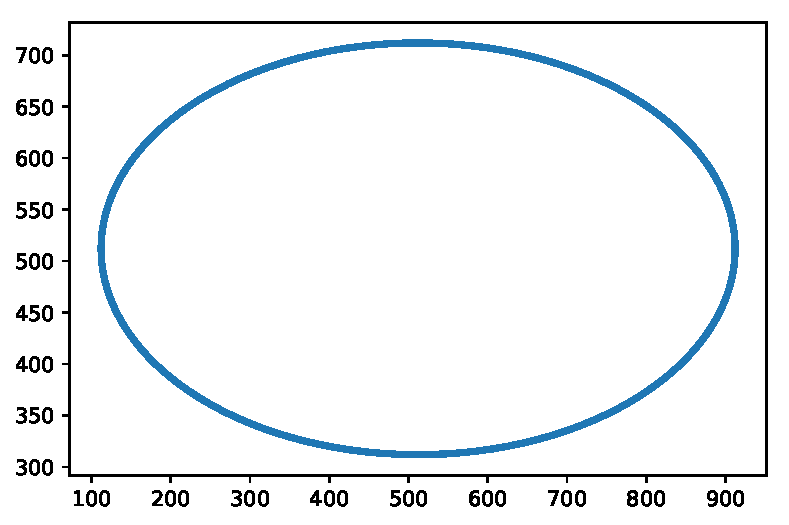
\includegraphics[width=.5\linewidth]{ellipse.pdf}%
 \label{fig:snakes:python:ellipse}%
\end{figure}

\vspace*{-10pt}

\subsection{Matrix construction}
This is maybe the hardest part of this code, with the use of the \pinline{scipy.sparse.diags} function.
\begin{python}
N = x.size;
X = np.array([-beta, alpha+4*beta, -2*alpha-6*beta, alpha+4*beta, -beta, -beta, alpha+4*beta, -beta, alpha+4*beta])
A = scipy.sparse.diags(X, np.array([-2, -1, 0, 1, 2, N-2, N-1, -N+2, -N+1]), shape=(N,N)).toarray();
AA = np.identity(N)-gamma*A;
invAA = np.linalg.inv(AA);
\end{python}

\subsection{External forces}
The external forces are computed with the following code. Notice that axis 0 correspond to the vertical axis (y) and and the axis 1 corresponds to the horizontal axis (x).
\begin{python}
# external forces computation
G = scipy.ndimage.filters.gaussian_gradient_magnitude(I, 30);
# Notice that horizontal axis x is 1, and vertical axis is 0
Fy = scipy.ndimage.prewitt(G, axis=0);
Fx = scipy.ndimage.prewitt(G, axis=1);
\end{python}

\subsection{Display results}
To enhance the role of the external forces, the arrows showing the force are displayed (\pinline{quiver} function, see Fig.\ref{fig:active_contours:python:forces}).

\begin{python}
imshow(I,[])
hold on
plot([x;x(1)], [y; y(1)], 'g', 'linewidth', 3);
# display arrows for external forces
step=20;
subx = 1:step:size(I,1);
suby = 1:step:size(I,2);
[Xa, Ya] = meshgrid(subx, suby);
quiver(Xa, Ya, Fx(subx, suby), Fy(subx,suby));
\end{python}

\begin{figure}[H]
 \centering\caption{External forces that will be applied to the snake.}%
 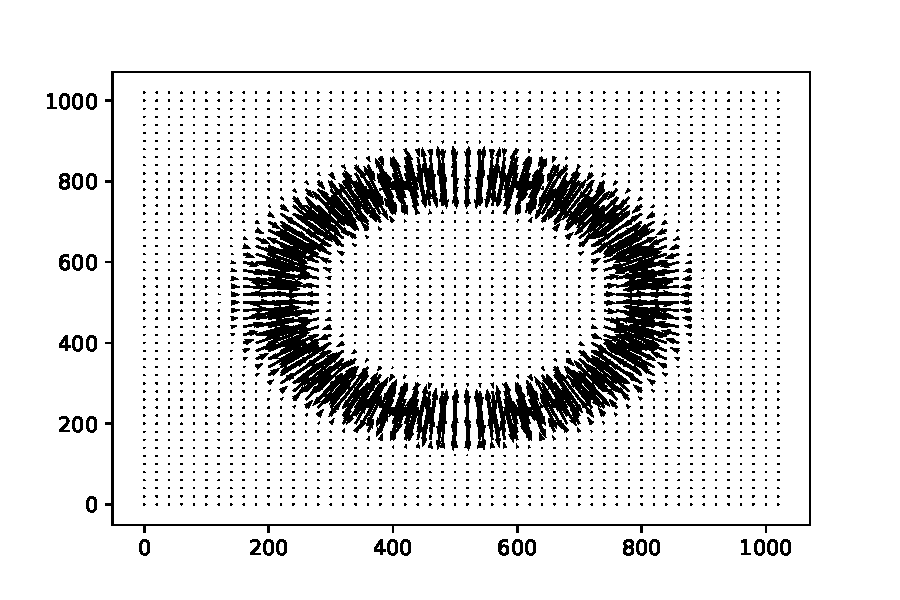
\includegraphics[width=.6\linewidth]{forces.python.pdf}%
 \label{fig:active_contours:python:forces}
\end{figure}

\vspace*{-10pt}

\subsection{Convergence algorithm}
\begin{python}
# interpolation methods to get values of the external forces at the 
# coordinates of the snake
sx, sy = I.shape;
ix = interpolate.interp2d(np.arange(n), np.arange(n), Fx);
iy = interpolate.interp2d(np.arange(n), np.arange(n), Fy);
# loop for convergence of the snake
bar = progressbar.ProgressBar();
for index in bar(range(iterations)):
    fex = np.array([float(ix(XX,YY)) for XX,YY in zip(x,y)]);
    fey = np.array([float(iy(XX,YY)) for XX,YY in zip(x,y)]);
    #print(np.max(fex), np.min(fex))
    x = np.matmul(invAA, x+gamma*fex);
    y = np.matmul(invAA, y+gamma*fey);
\end{python}

The results are displayed in Fig.\ref{fig:active_contours:python:result}.

\begin{figure}[H]
 \centering\caption{Result of the snake converging toward the disk, after 1000 iterations with the proposed parameters.}%
 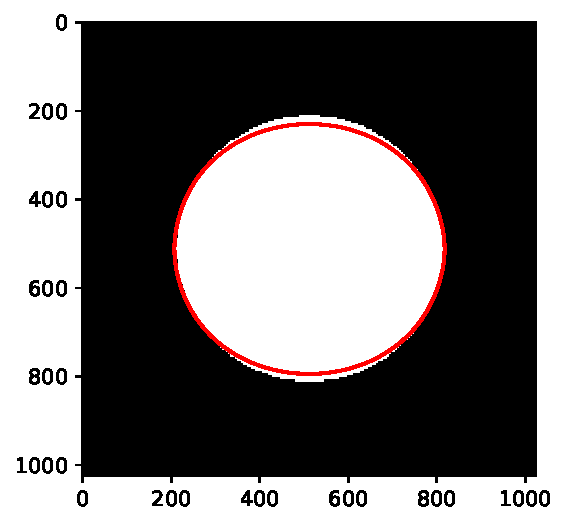
\includegraphics[width=.5\linewidth]{snake.python.pdf}%
 \label{fig:active_contours:python:result}%
\end{figure}
